  \chapter{Méthodologie et Conception du Système}
  \label{chap:methodologie}

  \section{Introduction}
  La conception d’un système capable de prédire le temps de cuisson des haricots à partir d’images s’inscrit dans une démarche méthodologique rigoureuse alliant vision par ordinateur, apprentissage automatique ultra-léger (TinyML) et pratiques expérimentales éprouvées. En combinant l’analyse non destructrice d’images à l’intégration dans des dispositifs à ressources limitées, ce travail vise à proposer une solution à la fois scientifiquement solide et technologiquement réalisable.

  Des études antérieures, utilisant l’imagerie hyperspectrale et la spectroscopie proche infrarouge (Vis/NIRS), ont démontré la capacité de modèles statistiques tels que la régression PLS à prédire avec une précision raisonnable le temps de cuisson de haricots trempés et non trempés (prédiction corrélée de \(R_{\text{pred}} \approx 0,886\) avec erreur standard \(\text{SEP} \approx 7,9\ \mathrm{min}\)) \autocite{mendoza2018}. Par ailleurs, l’adoption de systèmes TinyML dans des contextes industriels ou agroalimentaires a montré son potentiel pour des applications réactives, locales et éco-énergétiques \autocite{tinyml2024, emergingTinyML2025}.

  L’approche adoptée ici repose sur plusieurs étapes clés. D’abord, la collecte et le prétraitement d’un jeu de données d’images de haricots — incluant une variabilité de tailles, de textures et de conditions de cuisson — servent de fondation à la modélisation. Ensuite, nous évaluons des architectures adaptées aux contraintes embarquées, en partant d’un réseau convolutionnel léger jusqu’à des modèles préentraînés efficients tels que MobileNetV2. L’objectif est de réduire la lourdeur computationnelle tout en conservant une précision prédictive satisfaisante, à l’instar du modèle RecipeSnap, qui propose une réduction de plus de 70\% de la mémoire sans altérer la performance \autocite{recipesnap2022}.

  L’entraînement des modèles est conduit en tenant compte des bonnes pratiques : optimisation via Adam, régularisation (dropout, early stopping) et mesures objectives (MAE, RMSE, R², etc.). Enfin, une conversion en TensorFlow Lite (avec quantification en float16, int8) est effectuée pour obtenir une empreinte mémoire réduite, tout en testant l’inférence sur smartphone android — les travaux fondateurs de TensorFlow Lite Micro apportent un soutien technique précieux à cette étape \autocite{tfLiteMicro2020}.

  Cette méthodologie a pour ambition de proposer un pipeline complet, reproductible, allant de la capture d’images à la prédiction en temps réel sur smartphone android, afin de démontrer la faisabilité et l’efficacité de la vision par ordinateur embarquée dans le domaine agroalimentaire local.
 
 \begin{figure}[H]
  \centering
  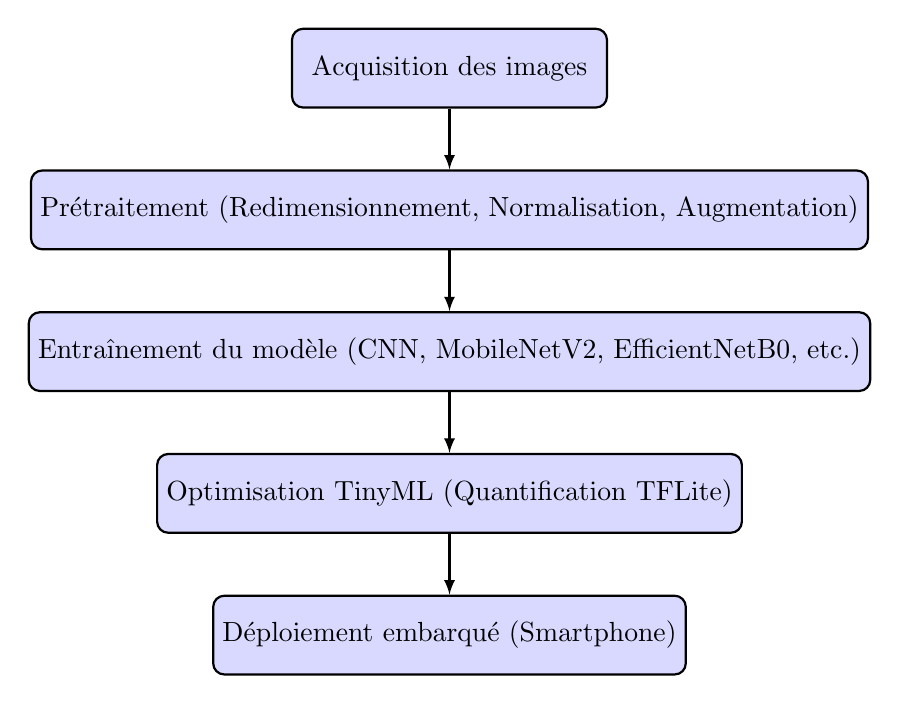
\begin{tikzpicture}[node distance=1.8cm, >=latex, thick]
      % Styles
      \tikzstyle{block} = [rectangle, draw=black, fill=blue!15, 
                          text centered, rounded corners, minimum width=4cm, minimum height=1cm]
      % Nodes
      \node[block] (acquisition) {Acquisition des images};
      \node[block, below of= acquisition] (pretraitement) {Prétraitement  (Redimensionnement, Normalisation, Augmentation)};
      \node[block, below of= pretraitement] (entrainement) {Entraînement du modèle  (CNN, MobileNetV2, EfficientNetB0, etc.)};
      \node[block, below of= entrainement] (optimisation) {Optimisation TinyML  (Quantification TFLite)};
      \node[block, below of= optimisation] (deploiement) {Déploiement embarqué  (Smartphone)};
      
      % Arrows
      \draw[->] (acquisition) -- (pretraitement);
      \draw[->] (pretraitement) -- (entrainement);
      \draw[->] (entrainement) -- (optimisation);
      \draw[->] (optimisation) -- (deploiement);
  \end{tikzpicture}
  \caption{Pipeline méthodologique proposé pour la prédiction du temps de cuisson des haricots basé sur TinyML.}
\end{figure}


  %%%%%%%%%%%%%%%%%%%%%%%%%%%%%%%%%%%%%%%%%%%%%%%%%%%%%%%%%%%%%%%%%%%%%%%%%%%%%%%%%%%%%%%%%%%%%%%%%%%%%%%%%%%%%%%%%%%%%%%%%%%%%%%%%%%%%%%%%%%%%%%%%%
  %%%%%%%%%%%%%%%%%%%%%%%%%%%%%%%%%%%%%%%%%%%%%%%%%%%%%%%%%%%%%%%%%%%%%%%%%%%%%%%%%%%%%%%%%%%%%%%%%%%%%%%%%%%%%%%%%%%%%%%%%%%%%%%%%%%%%%%%%%%%%%%%%%

  \section{Protocole expérimental — Prétraitement et préparation des jeux de données}

  Cette section détaille de façon exhaustive le protocole de prétraitement appliqué aux images et aux annotations de temps de cuisson ($T_c$), et précise la manière dont les jeux \emph{train/validation/test} sont construits et stockés pour l'entraînement et le déploiement TinyML.

  \subsection{Description synthétique du dataset source}

  Le jeu de données original comprend \(\mathbf{11\,200}\) images couleur au format JPEG, réparties équitablement sur \(\mathbf{8}\) variétés de haricots. Chaque variété est représentée par \(\mathbf{1\,400}\) images de haute résolution (\(3000\times4000\) pixels), répartie en \(\mathbf{7}\) sous-variétés contenant \(\mathbf{200}\) images chacune. Chaque image est associée à une annotation continue \(T_c\) (temps de cuisson en minutes), mesurée expérimentalement par chronométrage selon un protocole standardisé (arrêt au critère \emph{fork-tender}), avec une incertitude de mesure liée à l'opérateur estimée à \(\approx\pm 1\) minute.

  L’exploration préliminaire de la distribution des $T_c$ révèle une variabilité importante. Trois variétés présentent un pic de distribution autour de $120$ minutes, tandis que d'autres couvrent une plage de cuisson très large (approximativement de $70$ à $230$ minutes). Deux variétés en particulier montrent des profils de $T_c$ particulièrement étendus, ce qui souligne la nécessité d'une stratification rigoureuse lors du partitionnement des données pour garantir la représentativité de cette diversité dans chaque sous-ensemble.


  %%%%%%%%%%%%%%%%%%%%%%%%%%%%%%%%%%%%%%%%%%%%%%%%%%%%%%%%%%%%%%
  \subsection{Analyse Exploratoire et Statistiques Descriptives}

  Afin de caractériser quantitativement la distribution des données et d'orienter les choix de modélisation, une analyse exploratoire a été conduite \citep{tukey1977exploratory}. Cette analyse se concentre sur la distribution des temps de cuisson ($T_c$) à la fois globalement et au sein de chaque variété.

  %%%%%%%%%%%%%%%%%%%%%%%%%%%%%%%%%%%%%%%%%%%%%%%%%%%%%%%%%%%%%%
  \subsubsection{Statistiques descriptives par variété}

  Le tableau \ref{tab:stats_descriptives} résume les principaux descripteurs statistiques des temps de cuisson pour chaque variété.

  \begin{table}[!ht]
  \centering
  \caption{Statistiques descriptives des temps de cuisson ($T_c$ en minutes) par variété.}
  \label{tab:stats_descriptives}
  \begin{tabular}{lccccc}
  \toprule
  \textbf{Variété} & \textbf{Moyenne ($\mu$)} & \textbf{Écart-type ($\sigma$)} & \textbf{Min} & \textbf{Max} & \textbf{Effectif} \\ \midrule
  Dor701       & 145.86 & 72.67 & 62 & 280 & 1400 \\
  Escapan021   & 159.00 & 77.47 & 65 & 287 & 1400 \\
  GPL190C      & 160.00 & 74.19 & 70 & 295 & 1400 \\
  GPL190S      & 144.57 & 66.65 & 58 & 270 & 1400 \\
  Macc55       & 237.43 & 103.99 & 88 & 410 & 1400 \\
  NIT4G16187   & 118.86 & 45.18 & 68 & 210 & 1400 \\
  Senegalais   & 155.71 & 78.38 & 70 & 300 & 1400 \\
  TY339612     & 148.14 & 77.85 & 51 & 286 & 1400 \\ \bottomrule
  \end{tabular}
  \end{table}

  L'analyse de ces statistiques révèle plusieurs points cruciaux :
  \begin{itemize}
      \item \textbf{Forte hétérogénéité inter-variétés :} La moyenne des temps de cuisson varie considérablement, allant de $118.86$ min (NIT4G16187) à $237.43$ min (Macc55). Cette différence de plus de 100\% confirme que la variété est un facteur prédictif majeur du temps de cuisson.
      \item \textbf{Dispersion variable :} L'écart-type ($\sigma$), qui mesure la dispersion des valeurs autour de la moyenne, est également très hétérogène. La variété \texttt{Macc55} présente la plus forte dispersion ($\sigma \approx 104$ min), indiquant que ses temps de cuisson sont très étalés. À l'opposé, \texttt{NIT4G16187} est la plus homogène ($\sigma \approx 45$ min). Cette information est vitale : le modèle d'apprentissage pourrait avoir plus de difficultés à prédire avec précision le $T_c$ pour des variétés à forte variance.
      \item \textbf{Distribution globale :} La plage globale des temps de cuisson s'étend de 51 à 410 minutes, ce qui représente un défi de régression considérable pour un modèle TinyML contraint en ressources.
  \end{itemize}

  L'histogramme de la Figure \ref{fig:histogramme_tc} visualise la distribution globale des temps de cuisson, confirmant la présence de plusieurs modes et une asymétrie à droite.

  \begin{figure}[!ht]
  \centering
  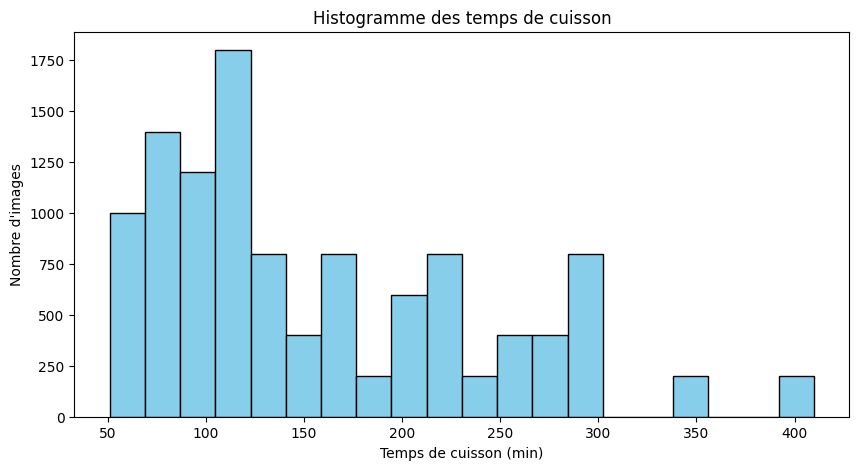
\includegraphics[width=0.8\textwidth]{figures/histogramme_tc.png}
  \caption{Distribution globale des temps de cuisson ($T_c$) pour l'ensemble des variétés. La distribution est multimodale, avec un pic principal autour de 120-150 minutes.}
  \label{fig:histogramme_tc}
  \end{figure}

  \subsubsection{Analyse de la variance intra-variété}

  Pour affiner l'analyse de la dispersion, la variance ($s^2 = \sigma^2$) a été calculée pour chaque variété (Tableau \ref{tab:variance_intra}). La variance quantifie la dispersion quadratique moyenne et accentue les différences de variabilité.

  \begin{table}[!ht]
  \centering
  \caption{Variance intra-variété des temps de cuisson.}
  \label{tab:variance_intra}
  \begin{tabular}{lc}
  \toprule
  \textbf{Variété} & \textbf{Variance Intra-variété ($s^2$)} \\ \midrule
  Dor701       & 5280.47 \\
  Escapan021   & 6002.00 \\
  GPL190C      & 5503.93 \\
  GPL190S      & 4442.28 \\
  Macc55       & 10813.97 \\
  NIT4G16187   & 2041.58 \\
  Senegalais   & 6143.16 \\
  TY339612     & 6060.17 \\ \bottomrule
  \end{tabular}
  \end{table}

  La Figure \ref{fig:boxplot_tc} (diagramme en boîtes à moustaches) offre une représentation visuelle comparative de ces variances. Elle met en évidence la médiane, l'intervalle interquartile (IQR) et l'étendue des données pour chaque catégorie, facilitant l'identification des distributions symétriques, asymétriques et des valeurs potentiellement aberrantes.

  \begin{figure}[!ht]
  \centering
  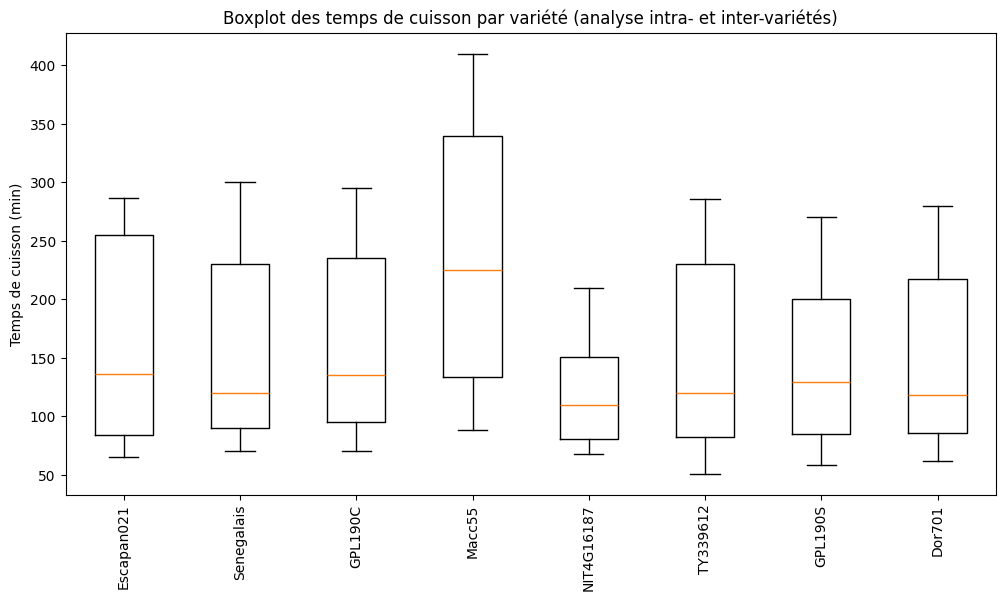
\includegraphics[width=0.9\textwidth]{figures/boxplot_tc.png}
  \caption{Diagramme en boîtes à moustaches illustrant la distribution des temps de cuisson par variété. La variabilité extrême de la variété \texttt{Macc55} et l'homogénéité de \texttt{NIT4G16187} sont clairement visibles.}
  \label{fig:boxplot_tc}
  \end{figure}

  L'examen de la variance et du boxplot confirme que la variété \texttt{Macc55} est un cas d'étude particulièrement difficile en raison de sa dispersion interne massive. Des facteurs non contrôlés, tels qu'une plus grande hétérogénéité génétique ou des conditions de croissance/stockage variables au sein de cette variété, pourraient expliquer ce phénomène. Du point de vue de la modélisation, cela implique que les caractéristiques visuelles extraites des images de \texttt{Macc55} doivent être particulièrement discriminantes pour permettre une régression précise.

  \subsubsection{Équilibre et distribution des données}

  La performance et l'impartialité d'un modèle d'apprentissage profond dépendent fortement de l'équilibre du jeu de données. La Figure \ref{fig:distrib_varietes} montre la répartition des échantillons par variété.

  \begin{figure}[!ht]
  \centering
  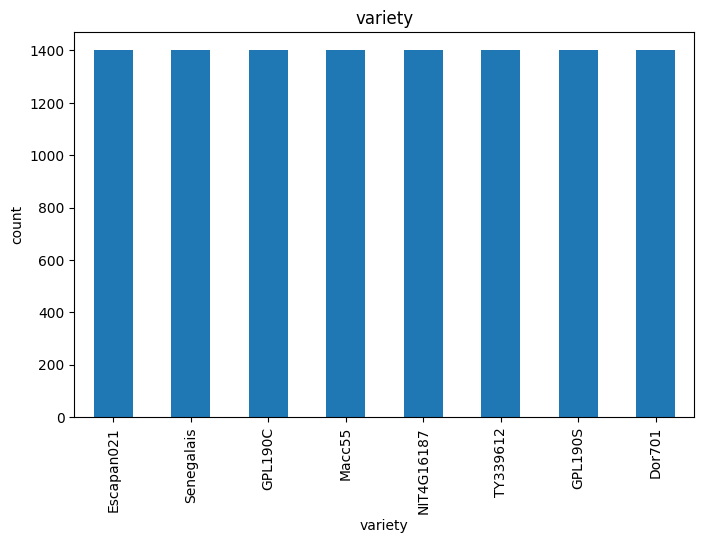
\includegraphics[width=0.7\textwidth]{figures/distrib_varietes.png}
  \caption{Distribution du nombre d'images par variété. Le jeu de données est parfaitement équilibré, chaque classe contenant 200 échantillons.}
  \label{fig:distrib_varietes}
  \end{figure}

  Le jeu de données est \textbf{parfaitement équilibré}, avec 200 images par variété. Cet équilibre est un atout majeur car il prévient tout biais du modèle en faveur des classes sur-représentées. La performance évaluée sera donc une juste réflexion de la capacité du modèle à généraliser sur toutes les variétés.


  \subsection{Pipeline de prétraitement}

  Le prétraitement appliqué aux images et aux annotations suit le pipeline illustré par la Figure \ref{fig:pipeline_preproc}. Seules les opérations jusqu'à l'enregistrement des jeux HDF5 sont incluses (préparation \textbf{offline} avant entraînement).

  \begin{figure}[H]
  \centering
  \begin{tikzpicture}[
    >=Latex,
    node distance=2.0cm,
    block/.style={rectangle, rounded corners=3pt, draw=black, fill=blue!12, align=center, minimum width=4.5cm, minimum height=0.9cm}
  ]
  \node[block] (raw) {Acquisition: images JPEG (3000×4000 px) \\ Labels: $T_c$ chronométrés};
  \node[block, below of=raw] (crop) {Recadrage centré / Ajustement d'exposition};
  \node[block, below of=crop] (resize) {Redimensionnement à 224×224 (PyTorch)};
  \node[block, below of=resize] (normalize_tc) {MinMax scaling de $T_c \to [0,1]$};
  \node[block, below of=normalize_tc] (augment) {Augmentation (train uniquement) $\times5$ \\ (flips, jitter, blur, noise)};
  \node[block, below of=augment] (h5) {Sauvegarde: un fichier HDF5 par split \\ clefs: \texttt{images}, \texttt{cooking\_times}};
  \draw[->] (raw) -- (crop);
  \draw[->] (crop) -- (resize);
  \draw[->] (resize) -- (normalize_tc);
  \draw[->] (normalize_tc) -- (augment);
  \draw[->] (augment) -- (h5);
  \end{tikzpicture}
  \caption{Pipeline de prétraitement des images et des labels $T_c$.}
  \label{fig:pipeline_preproc}
  \end{figure}

  \subsection{Redimensionnement et outils}

  Le redimensionnement est réalisé via \texttt{torchvision.transforms} (PyTorch) en appliquant un \texttt{CenterCrop} suivi d'un \texttt{Resize(224)} puis d'une normalisation des canaux si nécessaire pour des modèles pré-entraînés. Le choix $224\times224$ découle d'un compromis entre fidélité des motifs et coût mémoire d'inférence (MobileNetV2 / EfficientNet-B0 compatible) \citep{sandler2018mobilenetv2,krizhevsky2012imagenet}.

  \subsection{Augmentation (train uniquement) — paramètres}

  L'ensemble d'entraînement est étendu par un facteur $\mathbf{5}$ via des transformateurs aléatoires appliqués uniquement au split \emph{train} :
  \begin{itemize}
      \item \textbf{Flips horizontal et vertical} aléatoires ($p=0.5$),
      \item \textbf{RandomResizedCrop} (zoom et recadrage aléatoire),
      \item \textbf{ColorJitter} (variation de luminosité, contraste, saturation),
      \item \textbf{GaussianBlur} (flou gaussien léger),
      \item \textbf{Bruit Gaussien Additif}.
  \end{itemize}
  \textbf{Aucune rotation} n'est utilisée pour préserver les caractéristiques morphologiques directionnelles des grains. Ces transformations sont codées en PyTorch et appliquées stochastiquement pour générer quatre variantes supplémentaires par image d'entraînement initiale (1 image originale + 4 augmentées = facteur 5).

  \subsection{Normalisation des temps de cuisson ($T_c$)}

  Avant sauvegarde, les valeurs $T_c$ (en minutes) sont mises à l'échelle par la transformation \emph{Min–Max} pour produire une cible dans l'intervalle $[0,1]$. Formellement, les paramètres de la transformation sont calculés \textbf{uniquement} sur l'ensemble d'entraînement $\mathcal{D}_{\text{train}}$:

  \[
  T_{c,\min} = \min_{y\in \mathcal{D}_{\text{train}}} y, \qquad
  T_{c,\max} = \max_{y\in \mathcal{D}_{\text{train}}} y,
  \]
  \[
  \tilde{y} \;=\; \frac{y - T_{c,\min}}{T_{c,\max} - T_{c,\min}} \quad\in[0,1].
  \]

  Les mêmes $T_{c,\min}$ et $T_{c,\max}$ sont ensuite utilisés pour normaliser les ensembles de validation et de test, évitant ainsi toute fuite d'information du futur vers le modèle. Les valeurs prédites $\tilde{y}$ sont restaurées dans l'échelle d'origine (en minutes) par la transformation inverse $y = \tilde{y}\,(T_{c,\max}-T_{c,\min}) + T_{c,\min}$ lors de l'interprétation finale des résultats.

  \section{Conception du système proposé}

  La problématique adressée consiste à estimer, à partir d'une image unique d’un haricot (ou d'un petit lot représenté sur l'image), le temps de cuisson \(T_c\) exprimé en minutes. Le système doit être d'abord compétitif en termes de précision prédictive, puis contrainte à des ressources embarquées (smartphone et/ou microcontrôleur) via des techniques TinyML. La présente section décrit l'architecture générale et le pipeline de traitement, les modèles testés (deux CNN personnalisés et trois modèles préentraînés adaptés au mobile), les optimisations TinyML appliquées, ainsi que le workflow et l'architecture logicielle menant au déploiement.

  \subsection{Motivation et choix d'approche}

  L'approche par vision (images) est motivée par la possibilité d'extraire des indices visuels corrélés au temps de cuisson — couleur, taille, texture, proportion d'imperfections, etc. — sans recourir à des capteurs supplémentaires. Le passage à TinyML est justifié par l'objectif d'un service embarqué (hors-connexion) : confidentialité, latence faible et coût énergétique réduit. Les techniques d'optimisation (quantification, pruning, distillation) sont des bonnes pratiques largement documentées pour adapter des réseaux convolutifs classiques à des plateformes contraignantes \parencite{warden2019tinyml,Han2016DeepCompression}.

  \subsection{Architecture générale du modèle et pipeline}

  Le pipeline se décompose en quatre grandes phases (Figure~\ref{fig:pipeline}) :

  \begin{enumerate}
    \item \textbf{Prétraitement \& chargement} : lecture des HDF5, batch sampling, conversion en float32, normalisation canaux (mean/std) compatible avec les poids pré-entraînés ; augmentation appliquée uniquement au jeu d'entraînement.
    \item \textbf{Entraînement / Fine-tuning} : entraînement des CNN personnalisés depuis zéro et fine-tuning des modèles pré-entraînés (MobileNetV2, EfficientNet-B0, NASNetMobile) sur la tâche de régression continue (prévision du \(T_c\) normalisé).
    \item \textbf{Optimisation TinyML} : quantification (post-training et/ou quantization-aware training), pruning graduel, éventuellement distillation depuis un « teacher » plus large vers un « student » compact.
    \item \textbf{Déploiement \& mesures} : conversion en TFLite, mesures de latence et consommation sur smartphone cible (mesures empiriques, idéalement sur plusieurs appareils).
  \end{enumerate}

  \begin{figure}[!ht]
  \centering
  \begin{tikzpicture}[node distance=1.6cm, auto, >=Latex, thick]
  \tikzstyle{block} = [rectangle, rounded corners, draw, fill=blue!12, text centered, minimum height=1cm, minimum width=3.4cm]
  \node[block] (hdf5) {Chargement : HDF5 (train/val/test)};
  \node[block, below of=hdf5] (prep) {Normalisation des images};
  \node[block, below of=prep] (train) {Entraînement / Fine-tuning};
  \node[block, below of=train] (opt) {Quantification \& Pruning};
  \node[block, below of=opt] (deploy) {TFLite - Déploiement mobile};
  \draw[->] (hdf5) -- (prep);
  \draw[->] (prep) -- (train);
  \draw[->] (train) -- (opt);
  \draw[->] (opt) -- (deploy);
  \end{tikzpicture}
  \caption{Pipeline fonctionnel du système (chargement → entraînement → optimisation → déploiement).}
  \label{fig:pipeline}
  \end{figure}

  La fonction apprise s’écrit :
  \[
  \hat{T}_c = f_\theta\big(\mathcal{A}(I)\big)
  \]
  où \(I\in \mathbb{R}^{H\times W \times 3}\) est l'image d'entrée, \(\mathcal{A}\) l'opérateur de prétraitement (crop, resize à \(224\times224\), normalisation), et \(\theta\) les paramètres entraînés.

  \subsection{Description détaillée des modèles testés}

  Nous évaluons deux architectures convolutionnelles construites ad hoc (CNN-1 et CNN-2) et trois modèles mobiles pré-entraînés.

  \subsubsection{Formules de complexité et paramètres}

  Pour une couche convolutionnelle standard (sans séparabilité), le nombre de paramètres \(P\) et le nombre d'opérations élémentaires en multiplications-additions (FLOPs approximés par \emph{mult-adds}) pour une seule couche sont :
  \[
  P = (K \times K \times C_{in} + 1)\times C_{out},
  \]
  \[
  \text{FLOPs}_{\text{conv}} \approx 2 \times K \times K \times C_{in} \times C_{out} \times H_{out} \times W_{out},
  \]
  où \(K\) est la taille du noyau, \(C_{in},C_{out}\) canaux d'entrée/sortie et \(H_{out}\times W_{out}\) la résolution de la carte de caractéristiques en sortie (le facteur 2 approximant multiplication + addition). Pour les couches depthwise separable (utilisées par MobileNet), la complexité diminue sensiblement, ce qui explique l'efficacité de ces architectures sur mobile \citep{sandler2018mobilenetv2}.

  \subsubsection{CNN personnalisés (architectures fournies)}

\paragraph{CNN-1 TB-Net2 (profondeur progressive)}
L’architecture illustrée à la \textbf{Figure~\ref{fig:cnn1_tbnet2}} correspond à une approche dite de profondeur progressive, où le nombre de filtres est augmenté graduellement à mesure que la profondeur du réseau croît. Cette conception vise à extraire, dans un premier temps, des caractéristiques locales simples (bords, textures élémentaires), puis à capturer des représentations plus abstraites et discriminantes au fur et à mesure que les couches s’empilent.  

Chaque bloc convolutionnel est suivi d’une opération de sous-échantillonnage (\textit{MaxPooling2D}), qui réduit la résolution spatiale des cartes de caractéristiques tout en préservant les informations les plus saillantes. Cette stratégie permet de limiter la taille des tenseurs intermédiaires et d’augmenter l’invariance aux translations. L’intégration de couches de \textit{Dropout} avec un taux de 0.3 constitue un mécanisme de régularisation essentiel : elle réduit le risque de surapprentissage en introduisant une désactivation aléatoire de neurones lors de l’entraînement.  

Après plusieurs étapes de convolution et de pooling, une couche de \textit{GlobalAveragePooling2D} condense les cartes de caractéristiques en un vecteur représentatif, réduisant ainsi la dimensionnalité et favorisant la généralisation. Enfin, la partie dense est constituée d’une couche de 256 neurones activés par ReLU, suivie d’une couche de sortie unique adaptée à la régression du temps de cuisson.  

Dans l’ensemble, cette topologie offre un compromis pertinent entre expressivité et complexité computationnelle, en exploitant la profondeur pour raffiner progressivement l’information tout en maintenant une régularisation efficace.  

\begin{figure}[H]
    \centering
    \small
    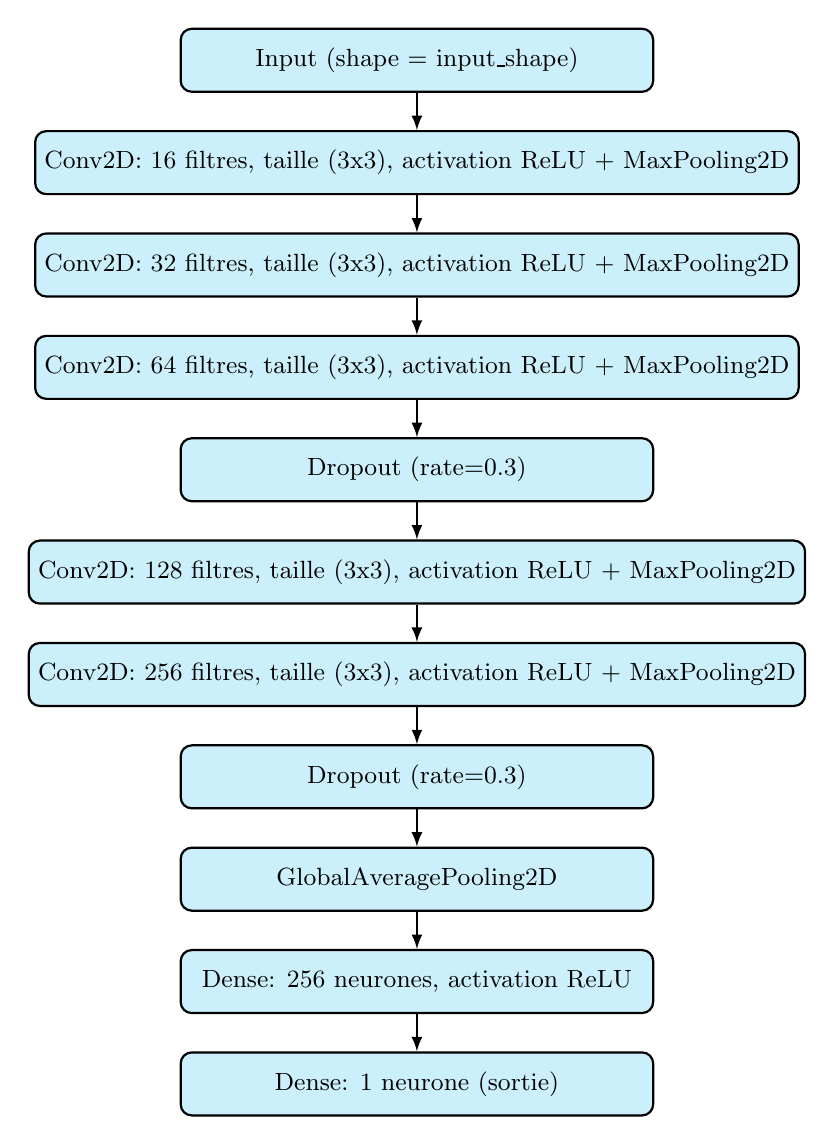
\begin{tikzpicture}[node distance=1.3cm, thick, >=latex, font=\small]
        \tikzstyle{block} = [rectangle, draw=black, fill=cyan!20, 
                            text centered, rounded corners, minimum width=6cm, minimum height=0.8cm]

        % Noeuds combinés Conv2D + MaxPooling2D
        \node[block] (input) {Input (shape = input\_shape)};
        \node[block, below of = input] (conv_pool1) {Conv2D: 16 filtres, taille (3x3), activation ReLU + MaxPooling2D};
        \node[block, below of = conv_pool1] (conv_pool2) {Conv2D: 32 filtres, taille (3x3), activation ReLU + MaxPooling2D};
        \node[block, below of = conv_pool2] (conv_pool3) {Conv2D: 64 filtres, taille (3x3), activation ReLU + MaxPooling2D};
        \node[block, below of = conv_pool3] (dropout1) {Dropout (rate=0.3)};
        \node[block, below of = dropout1] (conv_pool4) {Conv2D: 128 filtres, taille (3x3), activation ReLU + MaxPooling2D};
        \node[block, below of = conv_pool4] (conv_pool5) {Conv2D: 256 filtres, taille (3x3), activation ReLU + MaxPooling2D};
        \node[block, below of = conv_pool5] (dropout2) {Dropout (rate=0.3)};
        \node[block, below of = dropout2] (gap) {GlobalAveragePooling2D};
        \node[block, below of = gap] (dense1) {Dense: 256 neurones, activation ReLU};
        \node[block, below of = dense1] (output) {Dense: 1 neurone (sortie)};

        % Flèches
        \draw[->] (input) -- (conv_pool1);
        \draw[->] (conv_pool1) -- (conv_pool2);
        \draw[->] (conv_pool2) -- (conv_pool3);
        \draw[->] (conv_pool3) -- (dropout1);
        \draw[->] (dropout1) -- (conv_pool4);
        \draw[->] (conv_pool4) -- (conv_pool5);
        \draw[->] (conv_pool5) -- (dropout2);
        \draw[->] (dropout2) -- (gap);
        \draw[->] (gap) -- (dense1);
        \draw[->] (dense1) -- (output);
    \end{tikzpicture}
    \caption{Architecture CNN proposée avec blocs Conv2D et MaxPooling2D combinés.}
    \label{fig:cnn1_tbnet2_combined}
\end{figure}


\paragraph{CNN-2 TB-Net5 (bande passante accrue)}
L’architecture représentée à la \textbf{Figure~\ref{fig:cnn2_tbnet5}} se distingue du modèle précédent (CNN-1) par une augmentation significative de la largeur et de la profondeur des couches convolutionnelles. Alors que le premier réseau privilégiait une progression graduelle et régulière, ce second design adopte une stratégie d’expansion plus agressive du nombre de filtres, atteignant jusqu’à 512 dans les couches les plus profondes. Cette « bande passante accrue » confère au modèle une capacité de représentation plus riche, lui permettant de capturer des motifs complexes et subtils présents dans les images de haricots.  

Chaque bloc est constitué d’une couche \textit{Conv2D} suivie d’un \textit{MaxPooling2D}, assurant à la fois l’extraction de caractéristiques discriminantes et la réduction progressive de la résolution spatiale. La succession de ces blocs favorise une hiérarchisation efficace des représentations, allant des textures locales aux structures globales. L’intégration d’une couche de \textit{GlobalAveragePooling2D} avant la partie dense permet de condenser l’information tout en limitant la dimensionnalité des vecteurs de sortie.  

Enfin, une couche dense intermédiaire de 256 neurones activés par ReLU prépare les données avant la couche de sortie unique, adaptée à la régression du temps de cuisson. Bien que cette architecture soit plus coûteuse en termes de paramètres et d’opérations (FLOPs), elle est particulièrement pertinente lorsqu’une puissance de calcul suffisante est disponible, ou comme modèle « enseignant » dans une approche de distillation de connaissances en vue d’optimiser des variantes plus légères.  


\begin{figure}[H]
    \centering
    \small
    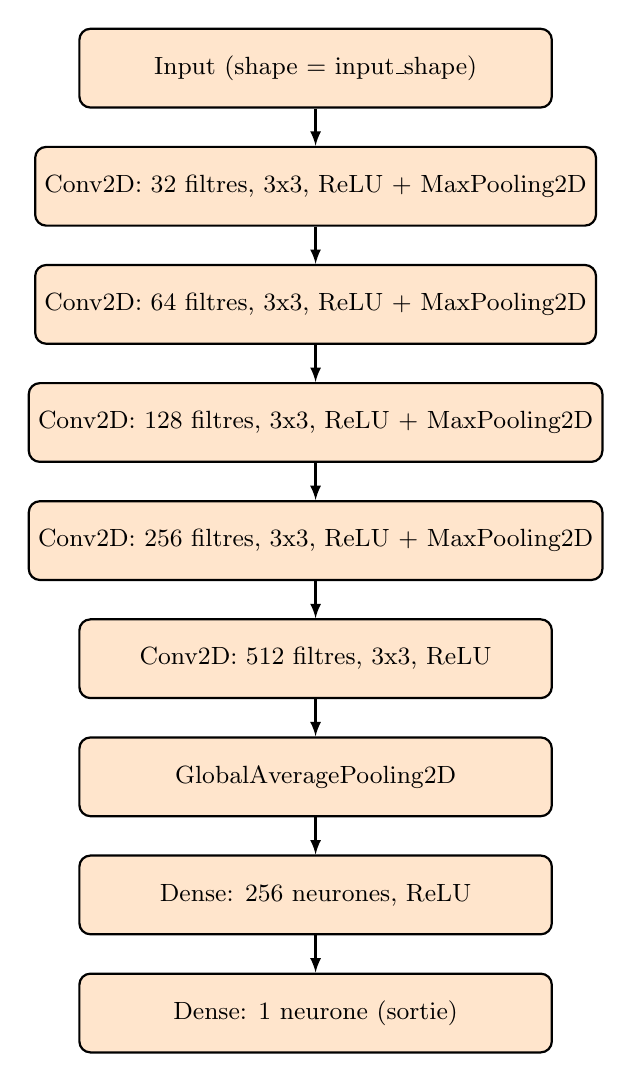
\begin{tikzpicture}[node distance=1.5cm, thick, >=latex, font=\small]
        \tikzstyle{block} = [rectangle, draw=black, fill=orange!20, 
                            text centered, rounded corners, minimum width=6cm, minimum height=1cm]

        % Noeuds combinés Conv2D + MaxPooling2D
        \node[block] (input) {Input (shape = input\_shape)};
        \node[block, below of = input] (conv_pool1) {Conv2D: 32 filtres, 3x3, ReLU + MaxPooling2D};
        \node[block, below of = conv_pool1] (conv_pool2) {Conv2D: 64 filtres, 3x3, ReLU + MaxPooling2D};
        \node[block, below of = conv_pool2] (conv_pool3) {Conv2D: 128 filtres, 3x3, ReLU + MaxPooling2D};
        \node[block, below of = conv_pool3] (conv_pool4) {Conv2D: 256 filtres, 3x3, ReLU + MaxPooling2D};
        \node[block, below of = conv_pool4] (conv5) {Conv2D: 512 filtres, 3x3, ReLU};
        \node[block, below of = conv5] (gap) {GlobalAveragePooling2D};
        \node[block, below of = gap] (dense1) {Dense: 256 neurones, ReLU};
        \node[block, below of = dense1] (output) {Dense: 1 neurone (sortie)};

        % Flèches
        \draw[->] (input) -- (conv_pool1);
        \draw[->] (conv_pool1) -- (conv_pool2);
        \draw[->] (conv_pool2) -- (conv_pool3);
        \draw[->] (conv_pool3) -- (conv_pool4);
        \draw[->] (conv_pool4) -- (conv5);
        \draw[->] (conv5) -- (gap);
        \draw[->] (gap) -- (dense1);
        \draw[->] (dense1) -- (output);
    \end{tikzpicture}
    \caption{Architecture CNN profonde avec blocs Conv2D et MaxPooling2D combinés.}
    \label{fig:cnn2_tbnet5_combined}
\end{figure}



  \subsubsection{Modèles pré-entraînés}

  \begin{itemize}
    \item \textbf{MobileNetV2} \parencite{sandler2018mobilenetv2} : architecture mobile employant des \emph{inverted residual} blocks et les convolutions séparables en profondeur ; MobileNetV2 (1.0, résolution 224) compte environ \(\mathbf{3.4M}\) paramètres et ~\(\mathbf{0.3}\) GFLOPs (mult-adds) pour une image 224×224, ce qui le rend très attractif pour l'embarqué.
    \item \textbf{EfficientNet-B0} \autocite{tan2019efficientnet} : conception via compound scaling ; EfficientNet-B0 : ~\(\mathbf{5.3M}\) paramètres et \(\approx\mathbf{0.39}\) GFLOPs (224×224). Excellente efficacité paramétrique/accuracie.
    \item \textbf{NASNetMobile} \autocite{zoph2018nasnet} : architecture trouvée par Neural Architecture Search pour des plateformes mobiles ; configurations compactes (taille et FLOPs compatibles avec mobile, ordre de quelques millions de paramètres selon l'implémentation).
  \end{itemize}

  Les nombres de paramètres et FLOPs cités ci-dessus proviennent des rapports originaux et benchmarks comparatifs (cf. Table~\ref{tab:model_comp} pour un résumé et les sources) \autocite{tan2019efficientnet,sandler2018mobilenetv2,zoph2018nasnet}.

  \subsection{Optimisations TinyML : quantification, pruning et techniques complémentaires}

  \subsubsection{Quantification}

  La quantification réduit la représentation numérique des poids et activations (fp32 → int8 ou fp16). La quantification post-training (PTQ) et la quantification-aware training (QAT) permettent d’obtenir des modèles 4× plus petits (int8) avec une perte de précision maîtrisée, surtout si l’on utilise une calibration dataset \autocite{jacob2018quantization,tensorflowlitequant}. TensorFlow Lite propose plusieurs variantes (dynamic range, full integer, float16) et outils pour mesurer l'impact \autocite{tensorflowlitequant}. 

  Mémoire approximative après quantification :
  \[
  \text{Taille}_{\text{int8}} \approx \frac{1}{4}\,\text{Taille}_{\text{fp32}}.
  \]
  Ex. : modèle fp32 12\,MiB \(\rightarrow\) int8 \(\approx\) 3\,MiB.

  \subsubsection{Pruning (élagage)}

  Le pruning structurel ou non-structurel supprime des poids ou canaux peu contributifs. En pratique, on applique un schéma de pruning itératif pendant l'entraînement et un ré-entraînement (fine-tuning) après pruning pour récupérer la performance \autocite{hinton2015distillation}. Les gains en mémoire et latence dépendent fortement de l'implémentation matérielle (le pruning non-structuré n'est pas toujours accéléré par le matériel généraliste).

  \subsubsection{Distillation de connaissances}

  Pour réduire davantage la taille tout en conservant la performance, on peut distiller un réseau compact (student) à partir d'un réseau plus large (teacher) — méthode particulièrement utile si l’on entraîne un petit CNN (CNN-2 ou CNN-1 après pruning) pour produire un modèle embarquable \autocite{hinton2015distillation}.

  \subsection{Workflow expérimental et hyperparamètres}

  Nous suivons une procédure reproductible incluant des scripts d'entraînement, conversion et test. Le tableau~\ref{tab:hyper} résume les hyperparamètres recommandés pour l'expérimentation initiale ; ces valeurs servent de baseline et peuvent être optimisées par recherche (grid/random/Bayesian).

  \begin{table}[!ht]
  \centering
  \caption{Hyperparamètres d'entraînement recommandés.}
  \label{tab:hyper}
  \resizebox{\textwidth}{!}{%
  \begin{tabular}{@{}lcc@{}}
  \toprule
  Hyperparamètre & Valeur (baseline) & Commentaire \\ \midrule
  Batch size & 32 & adapter selon VRAM GPU \\
  Optimiseur & Adam & \(\beta_1=0.9, \beta_2=0.999\) \\
  Learning rate init. & $10^{-4}$ & scheduler Cosine decay ou ReduceOnPlateau \\
  Epochs & 100 & early stopping sur val loss (patience 5) \\
  Loss & MSE (régression) & on suit MAE/MAPE en métriques secondaires \\
  Augmentation (train) & flip, crop, color jitter, blur, bruit gaussien & multiplicateur ×5 \\
  Normalisation sorties & Min–Max (train) & transforme \(T_c\) en \([0,1]\) \\
  Quantification & PTQ int8 puis QAT si forte dégradation & calibration sur subset test \\
  Pruning & 30–60\% sparsité progressive & ré-entraînement post-pruning \\
  \bottomrule
  \end{tabular}%
  }
  \end{table}


  \subsection{Comparaison chxiffrée des modèles (estimation)}

  La Table~\ref{tab:model_comp} rassemble des métriques utiles pour comparer précision/complexité/taille : nombre de paramètres, FLOPs (mult-adds), taille indicative après quantification en int8, et latence attendue (estimation à valider empiriquement sur smartphone cible). Les valeurs de paramètres/FLOPs sont extraites des publications originales et benchmarks \autocite{sandler2018mobilenetv2,tan2019efficientnet,zoph2018nasnet, openbenchmarks}.

  \begin{table}[!ht]
  \centering
  \caption{Comparatif des modèles (valeurs indicatives pour 224×224).}
  \label{tab:model_comp}
  \begin{tabular}{@{}lcccc@{}}
  \toprule
  Modèle & \# Param. & FLOPs (G) & Taille float16 (est.) & Latence \\
  & (M) & (mult-adds) & (Mo) & (ms sur smartphone) \\ \midrule
  CNN-1 (config) &  \(\approx\) 1.38 & \(\approx\) 0.1 & 0.90 & 20--30\(^\dagger\) \\
  CNN-2 (config) &  \(\approx\) 5 & \(\sim\) 0.4--0.6 & 5 & 40--80\(^\dagger\) \\
  MobileNetV2 (1.0) & \(\approx\) 3.4 & \(\approx\) 0.3 & \(\approx\) 2.4--6.6 & 30--60\(^\dagger\) \\
  EfficientNet-B0 & \(\approx\) 5.3 & \(\approx\) 0.39 & \(\approx\) 2.8--5.5 & 40--80\(^\dagger\) \\
  NASNetMobile & \(\sim\) 4.0--6.0 & \(\sim\) 0.5--0.6 & \(\approx\) 3.0--7.0 & 50--100\(^\dagger\) \\ \bottomrule
  \end{tabular}
  \begin{flushleft}
  \footnotesize{\(^\dagger\) latences approximatives — très dépendantes du modèle exact, du téléphone (CPU, NNAPI), et de la présence d'accélération intégée. Mesures empiriques recommandées (cf. \autocite{tan2019efficientnet,sandler2018mobilenetv2,tan2019mnasnet}).}
  \end{flushleft}
  \end{table}

  \noindent \textbf{Note importante :} les chiffres indiqués sont des ordres de grandeur tirés de la littérature et de benchmarks publics ; il est impératif de mesurer la latence et la consommation sur la plateforme cible (par ex. instrumentation via Android Profiler, Systrace, ou outils d’energy profiling) pour obtenir des valeurs applicables \autocite{tan2019mnasnet}.

  \subsection{Intégration embarquée : smartphone, gestion mémoire, latence et consommation}

  \paragraph{Plateforme cible}  
  Le choix initial est le smartphone Android moderne (API >= 24) afin d'utiliser TensorFlow Lite et NNAPI pour l'accélération. Pour microcontrôleurs, la chaîne change (TFLite Micro, contraintes SRAM/Flash beaucoup plus strictes) ; Warden et Situnayake fournissent des guides pratiques pour Arduino/MCU \autocite{warden2019tinyml}.

  \paragraph{Mesures et profilage}  
  Mesures empiriques à effectuer :
  \begin{itemize}
    \item \textbf{Taille binaire du modèle} (apk ou fichier .tflite) avant/après quantification ;
    \item \textbf{Latence d'inférence} (cold start et warm runs) : moyenne et percentiles sur N exécutions ;
    \item \textbf{Consommation énergétique} (mJ) par inférence : via instrumentation matérielle (moniteur de courant) ou outils logicielles approximatives ;
    \item \textbf{Utilisation mémoire} (heap et allocation interne du runtime).
  \end{itemize}
  Ces mesures servent à comparer les modèles et à choisir le meilleur compromis précision/consommation/latence \autocite{tan2019mnasnet,fbnet}.

  \paragraph{Gestion mémoire et performance}  
  Quelques bonnes pratiques pour réduire l'empreinte :
  \begin{itemize}
    \item utiliser \texttt{delegate} matériels (NNAPI, GPU delegate) quand disponibles ;
    \item privilégier la quantification entière (int8) pour la réactivité CPU et la réduction mémoire \autocite{jacob2018quantization,tensorflowlitequant};
    \item s'assurer que les buffers d'entrée/sortie sont réutilisés pour éviter des allocations répétées ;
    \item appliquer pruning structurel pour réduire latence (canaux/filters pruning) plutôt que pruning non-structuré si l'accélération matérielle est limitée.
  \end{itemize}

  \subsection{Aspects reproductibilité et intégration continue}

  Le pipeline CI doit inclure :
  \begin{itemize}
    \item scripts pour recréer dataset HDF5 à partir des images (même random seed pour splits) ;
    \item étapes d'entraînement avec logging (TensorBoard), sauvegarde de checkpoints et export du modèle sauvegardé ;
    \item étapes automatisées de conversion TFLite + application des options de quantification (scripts identiques à ceux utilisés pour la production) ;
    \item tests unitaires validant que la sortie TFLite réplique la prédiction du modèle de référence (tolérance via MAE).
  \end{itemize}

  \subsection{Discussion critique et limites}

  \begin{itemize}
    \item \textbf{Variabilité inter-variétés} : la distribution des temps de cuisson varie fortement selon la variété (cf. protocole). Un modèle global peut sous-performer pour certaines variétés ; des stratégies incluent l'ajout d'un embedding de variété (si l'information est connue) ou l'entraînement de modèles spécialisés.
    \item \textbf{Sources d'erreur visuelle} : éclairage, positionnement, ombres peuvent dégrader les prédictions ; inclure des augmentations robustes et collecter des images représentatives en conditions réelles réduit ce risque.
    \item \textbf{Compromis précision/latence} : une petite perte de précision peut être acceptable si la latence et la consommation chutent significativement — décision à prendre selon contrainte d'usage (temps réel vs analyse batch).
  \end{itemize}

  La conception exposée ci-dessus fixe les choix techniques et les métriques d'évaluation nécessaires. Le chapitre suivant (Implémentation) détaillera la configuration expérimentale (scripts d'entraînement Keras/TensorFlow), les commandes de conversion TFLite (options de quantification), les protocoles de mesure sur smartphone et les résultats empiriques (MAE, RMSE, taille finale des modèles, latence et consommation mesurées).